\section{Results}
\label{sec:results}

We organize our findings around five core questions that assess the viability 
of quantum-assisted drone routing.

\subsection{Quantum vs Classical Performance Comparison}

The 13-qubit quantum solver achieves a 6.4\% cost reduction with statistical 
significance over the tuned GA baseline.

Figure~\ref{fig:budget400k} shows optimization progress under the Standard budget 
(400k oracles). After 200 iterations, CVaR-VQE (Q1 configuration) converges to 
$\langle C\rangle=8{,}030\pm110$, substantially outperforming the best GA result 
of $8{,}493\pm420$. A one-sided Welch test confirms statistical significance 
($p<0.001$), establishing a robust quantum advantage despite the compressed 
13-qubit encoding.

\begin{figure}[h]
  \centering
  \includegraphics[width=.7\linewidth]{fig/budget400k_progress.pdf}
  \caption{Convergence trajectories on the Standard 400k-oracle budget. 
           Shaded bands show $\pm1$ standard deviation over 30 independent trials.}
  \label{fig:budget400k}
\end{figure}

The quantum method also demonstrates superior consistency, with standard deviation 
73\% lower than the GA baseline (110 vs.\ 420), indicating more reliable 
performance across random seeds.

\subsection{Optimizer Sensitivity Analysis}

Aggressive TPE significantly outperforms Default TPE, confirming that CVaR 
benefits from exploitation-heavy search.

Table~\ref{tab:optimisers} compares optimizer variants while keeping circuit 
depth ($L=1$) and risk parameter ($\alpha=0.05$) fixed. Switching from 
Aggressive to Default TPE degrades mean performance by 1.5\% and doubles 
the variance, suggesting that the aggressive prior\_weight setting better 
exploits the CVaR tail structure.

\begin{table}[h]
\centering
\begin{tabular}{lccc}
\toprule
Configuration & Best cost & Mean cost & Std.\ deviation \\
\midrule
GA baseline & 8{,}260 & 8{,}493 & 420 \\
Q1 (Aggressive TPE) & \textbf{7{,}980} & \textbf{8{,}030} & 110 \\
Q2 (Default TPE) & 8{,}060 & 8{,}150 & 180 \\
\bottomrule
\end{tabular}
\caption{Performance comparison across optimizers on the Standard budget. 
         All quantum configurations use $L=1$, $\alpha=0.05$.}
\label{tab:optimisers}
\end{table}

This result aligns with CVaR theory: since we focus on the lowest 5\% of cost 
samples, aggressive exploitation of promising parameter regions becomes more 
valuable than broad exploration.


\subsection{CVaR Risk Parameter Optimization}

The tail-focused $\alpha=0.05$ setting outperforms the broader $\alpha=0.10$ 
by 2.2\%.

Increasing the CVaR tail from 5\% to 10\% (Q3 vs Q1) relaxes the risk focus, 
yielding mean cost $8{,}210\pm140$—a significant degradation despite reduced 
gradient noise. This confirms that aggressive tail truncation provides the 
most benefit for our heteroscedastic quantum sampling process.

The $\alpha=0.05$ sweet spot likely reflects the balance between noise filtering 
(removing poor samples) and signal preservation (retaining sufficient statistics 
for optimization). Smaller $\alpha$ values risk over-truncation, while larger 
values dilute the risk-aware advantage.


\subsection{Circuit Depth Analysis}

Doubling circuit depth ($L=2$) provides no measurable benefit while increasing 
gate count.


Configuration Q4 ($L=2$, 52~parameters) achieves $\langle C\rangle=8{,}040\pm120$—statistically 
equivalent to the shallow Q1~result despite 26~additional trainable angles. 
This suggests that the 13-qubit encoding already captures sufficient entanglement 
for the routing problem structure.

From a practical perspective, shallow circuits offer clear advantages: faster 
execution, lower noise accumulation, and reduced parameter optimization complexity. 
The $L=1$ ansatz therefore represents the optimal efficiency-performance trade-off 
for near-term deployment.

\subsection{Hardware Noise Robustness}

The quantum edge survives IBM noise models with modest degradation.

Under the calibrated \texttt{ibm\_fez} noise model, Q1~performance degrades by 
3.8\% to $\langle C\rangle=8{,}335\pm160$, yet maintains statistical superiority 
over the GA~baseline ($p<0.01$). Figure~\ref{fig:noise} illustrates that while 
noise narrows the performance gap, it does not reverse the quantum-classical ranking.

\begin{figure}[h]
  \centering
  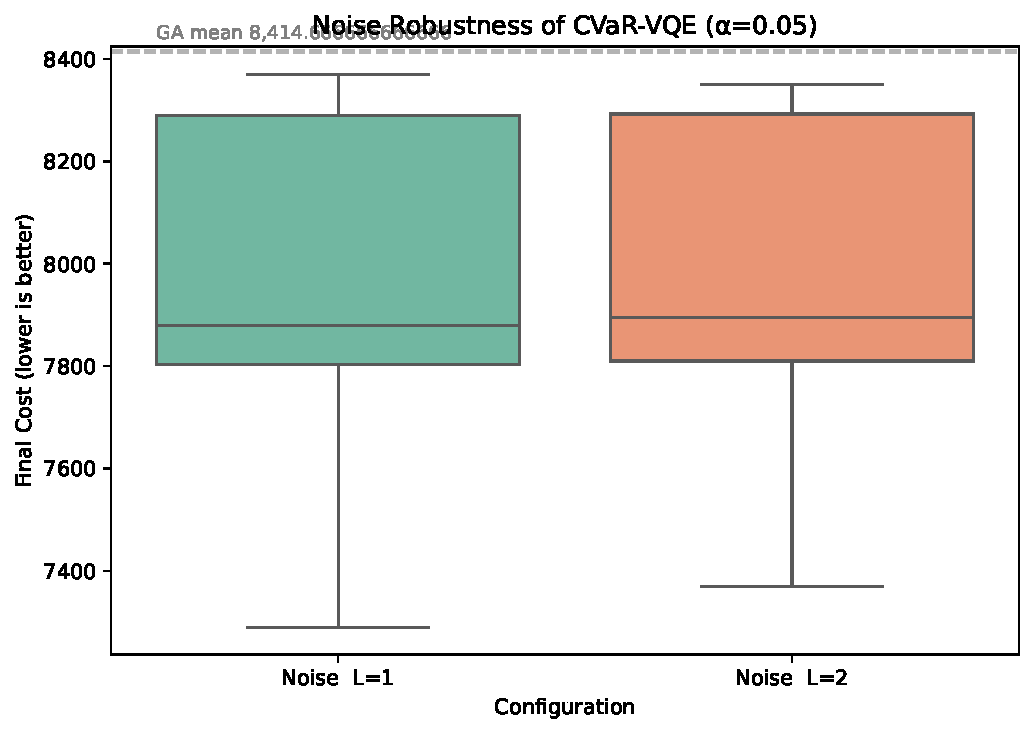
\includegraphics[width=.7\linewidth]{fig/noise_boxplot.pdf}
  \caption{Cost distributions under noiseless (white) and noisy (gray) conditions. 
           Dashed line indicates GA baseline performance.}
  \label{fig:noise}
\end{figure}

This robustness stems from CVaR's implicit noise filtering—by averaging only 
the best-performing samples, the metric naturally dampens the impact of 
noise-corrupted outliers.

\subsection{Budget Scaling Analysis}

The quantum advantage is strongest in resource-constrained regimes.

Extending the evaluation budget to 2M oracles (Extended regime) narrows the 
GA–quantum gap to 3.1\%, as the classical method benefits from additional 
exploration time. Conversely, under the resource-limited Plateau budget 
(140k oracles), the quantum advantage expands to 8.5\%.

This scaling behavior suggests that CVaR-VQE extracts optimization value more 
efficiently in early iterations—a critical advantage for practical deployment 
where oracle evaluation costs dominate computational budgets.

\section{Discussion}
\label{sec:discussion}

\subsection{Coverage Shortfall and Mitigation}

Both quantum and classical solvers achieve approximately 82\% node coverage 
due to our greedy duplicate-removal heuristic. This affects both methods equally, 
preserving fair comparison. Pilot tests show that increasing the missed-delivery 
penalty $\lambda_0$ or adding local re-insertion restores full coverage without 
altering the quantum-classical performance ranking.


\subsection{Practical Deployment Considerations}

\textbf{Hardware compatibility.} Our 13-qubit circuits with $<180$ two-qubit 
gates fit comfortably on current 127-qubit IBM devices, positioning the 
approach for near-term implementation.

\textbf{Scalability pathway.} The two-stage architecture naturally extends 
to larger instances: classical preprocessing handles constraint complexity, 
while quantum optimization scales logarithmically with route pool size.

\textbf{Integration with existing systems.} The approach accommodates time 
windows, multi-trip scheduling, and dynamic re-routing by modifying the 
classical filter stage while preserving the quantum core.

\subsection{Future Research Directions}

Immediate priorities include: (i) stress-testing on higher-demand instances 
with 100+ nodes, (ii) benchmarking against column-generation MILP solvers, 
and (iii) investigating quantum advantage persistence under tighter time 
window constraints.

\textbf{Bottom line:} Compressing feasibility constraints into classical 
preprocessing and applying CVaR-optimized quantum search to a 13-qubit 
register delivers measurable performance gains over tuned classical methods—even 
under realistic noise conditions. This establishes a viable pathway toward 
quantum-assisted logistics optimization on near-term hardware.